\documentclass{article}
\title{Intro to PDEs: Ch 4.1-4.2 HW}
\author{Logan Rhyne, Harley Combest, Roy Galang, Jesse DiCenso}
\usepackage[T1]{fontenc}
\usepackage{amsfonts, amsmath, amsthm, amssymb}
\usepackage{mathtools, bigints, empheq}
\usepackage{graphicx, wrapfig, xcolor, float}
\usepackage{stackrel}
\usepackage{pgfplots}
\usepackage[shortlabels]{enumitem}
\usepackage[margin=1.0in]{geometry}
\setlength{\parindent}{0pt}
\theoremstyle{definition}
\newtheorem*{lemma}{Lemma}
\newtheorem*{conj}{Conjecture}
\newtheorem{prob}{}
\newtheorem*{pf}{Proof}
\newtheorem*{dpf}{Disproof}
\renewcommand\qedsymbol{$\blacksquare$}
\renewcommand{\emptyset}{\varnothing}
\renewcommand{\epsilon}{\varepsilon}
\newenvironment{disproof}{\begin{proof}[Disproof]}{\end{proof}}
\newenvironment{ans}{\begin{proof}[Answer]\renewcommand{\qedsymbol}{}}{\end{proof}}
\newenvironment{boldenv}{\bfseries\boldmath}{}
\newcommand{\N}{\mathbb{N}}
\newcommand{\Z}{\mathbb{Z}}
\newcommand{\R}{\mathbb{R}}

\pgfplotsset{compat=1.18}

\DeclareMathOperator{\ran}{range}

\begin{document}

\maketitle

"Solve equation graphically" means that you plot a corresponding function and points $(z_n , 0)$ where it intersects with $OX$ will give us all the frequencies $\omega_n = \omega (z_n)$.

"Simple solution" $u(x,t)=X(x)T(t)$.

\textbf{Hint.} You may assume that all eigenvalues are real (which is the case). In Problems 3-8 \emph{(note: for this assignment, this will just concern problems 3 and 4)} you may assume that all eigenvalues are real and non-negative (which is also the case).

\begin{boldenv}
    \underline{Problem 1}. Justify Example 4.2.6 and Example 4.mathjax/2.7.5: Consider eigenvalue problem with Robin boundary conditions
    \begin{align}
        &X''+\lambda X=0 \mkern 50mu 0<x<l,\\
        &X'(0)=\alpha X(0),\\
        &X'(l)=-\beta X(l)
    \end{align}
    with $\alpha, \beta \in \R$. \begin{enumerate}
        \item Prove that positive eigenvalues are $\lambda_n = \omega_n^2$ and the corresponding eigenfunctions are $X_n$ where $\omega_n > 0$ are roots of
        \begin{align}
            \tan{(\omega l)} &= \frac{(\alpha + \beta)\omega}{\omega^2 - \alpha \beta}\\
            X_n &= \omega_n \cos{(\omega_n x)} + \alpha \sin{(\omega_n x)}
        \end{align}

        \item Prove that negative eigenvalues if there are any are $\lambda_n = -\gamma_n^2$ and the corresponding eigenfunctions are $Y_n \text{ where } \gamma_n > 0$ are roots of
        \begin{align}
            \tan{(\gamma l)} &= -\frac{(\alpha + \beta)\gamma}{\gamma^2 - \alpha \beta}\\
            Y_n &= \gamma_n \cosh{(\gamma_n x)} + \alpha \sin{(\gamma_n x)}
        \end{align}
        Solve this equation graphically.

        \item To investigate how many negative eigenvalues are, consider the threshold case of eigenvalue $\lambda = 0$: then $X = cx+d$ and plugging into b.c. we have $c=\alpha d$ and $c=-\beta (d+lc)$; this system has non-trivial solution $(c,d) \neq 0$ iff $\alpha + \beta + \alpha \beta l =0$. This hyperbola divides $(\alpha , \beta)$-plane into three zones.

        \item Prove that eigenfunctions corresponding to different eigenvalues are orthogonal:
        \[ \int_0^l X_n(x)X_m(x)\,dx = 0 \mkern 50mu \text{ as } \lambda_n \neq \lambda_m \]
        where we consider now all eigenfunctions (no matter corresponding to positive or negative eigenvalues).

    \end{enumerate}
\end{boldenv}
\begin{ans}
    \begin{enumerate}
        \item \phantom{.}
        \begin{figure}[H]
            \centering
            \includegraphics[width=0.3\textwidth]{Problem 1-1.jpeg}
            \includegraphics[width=0.3\textwidth]{Problem 1-1 (2).jpeg}
            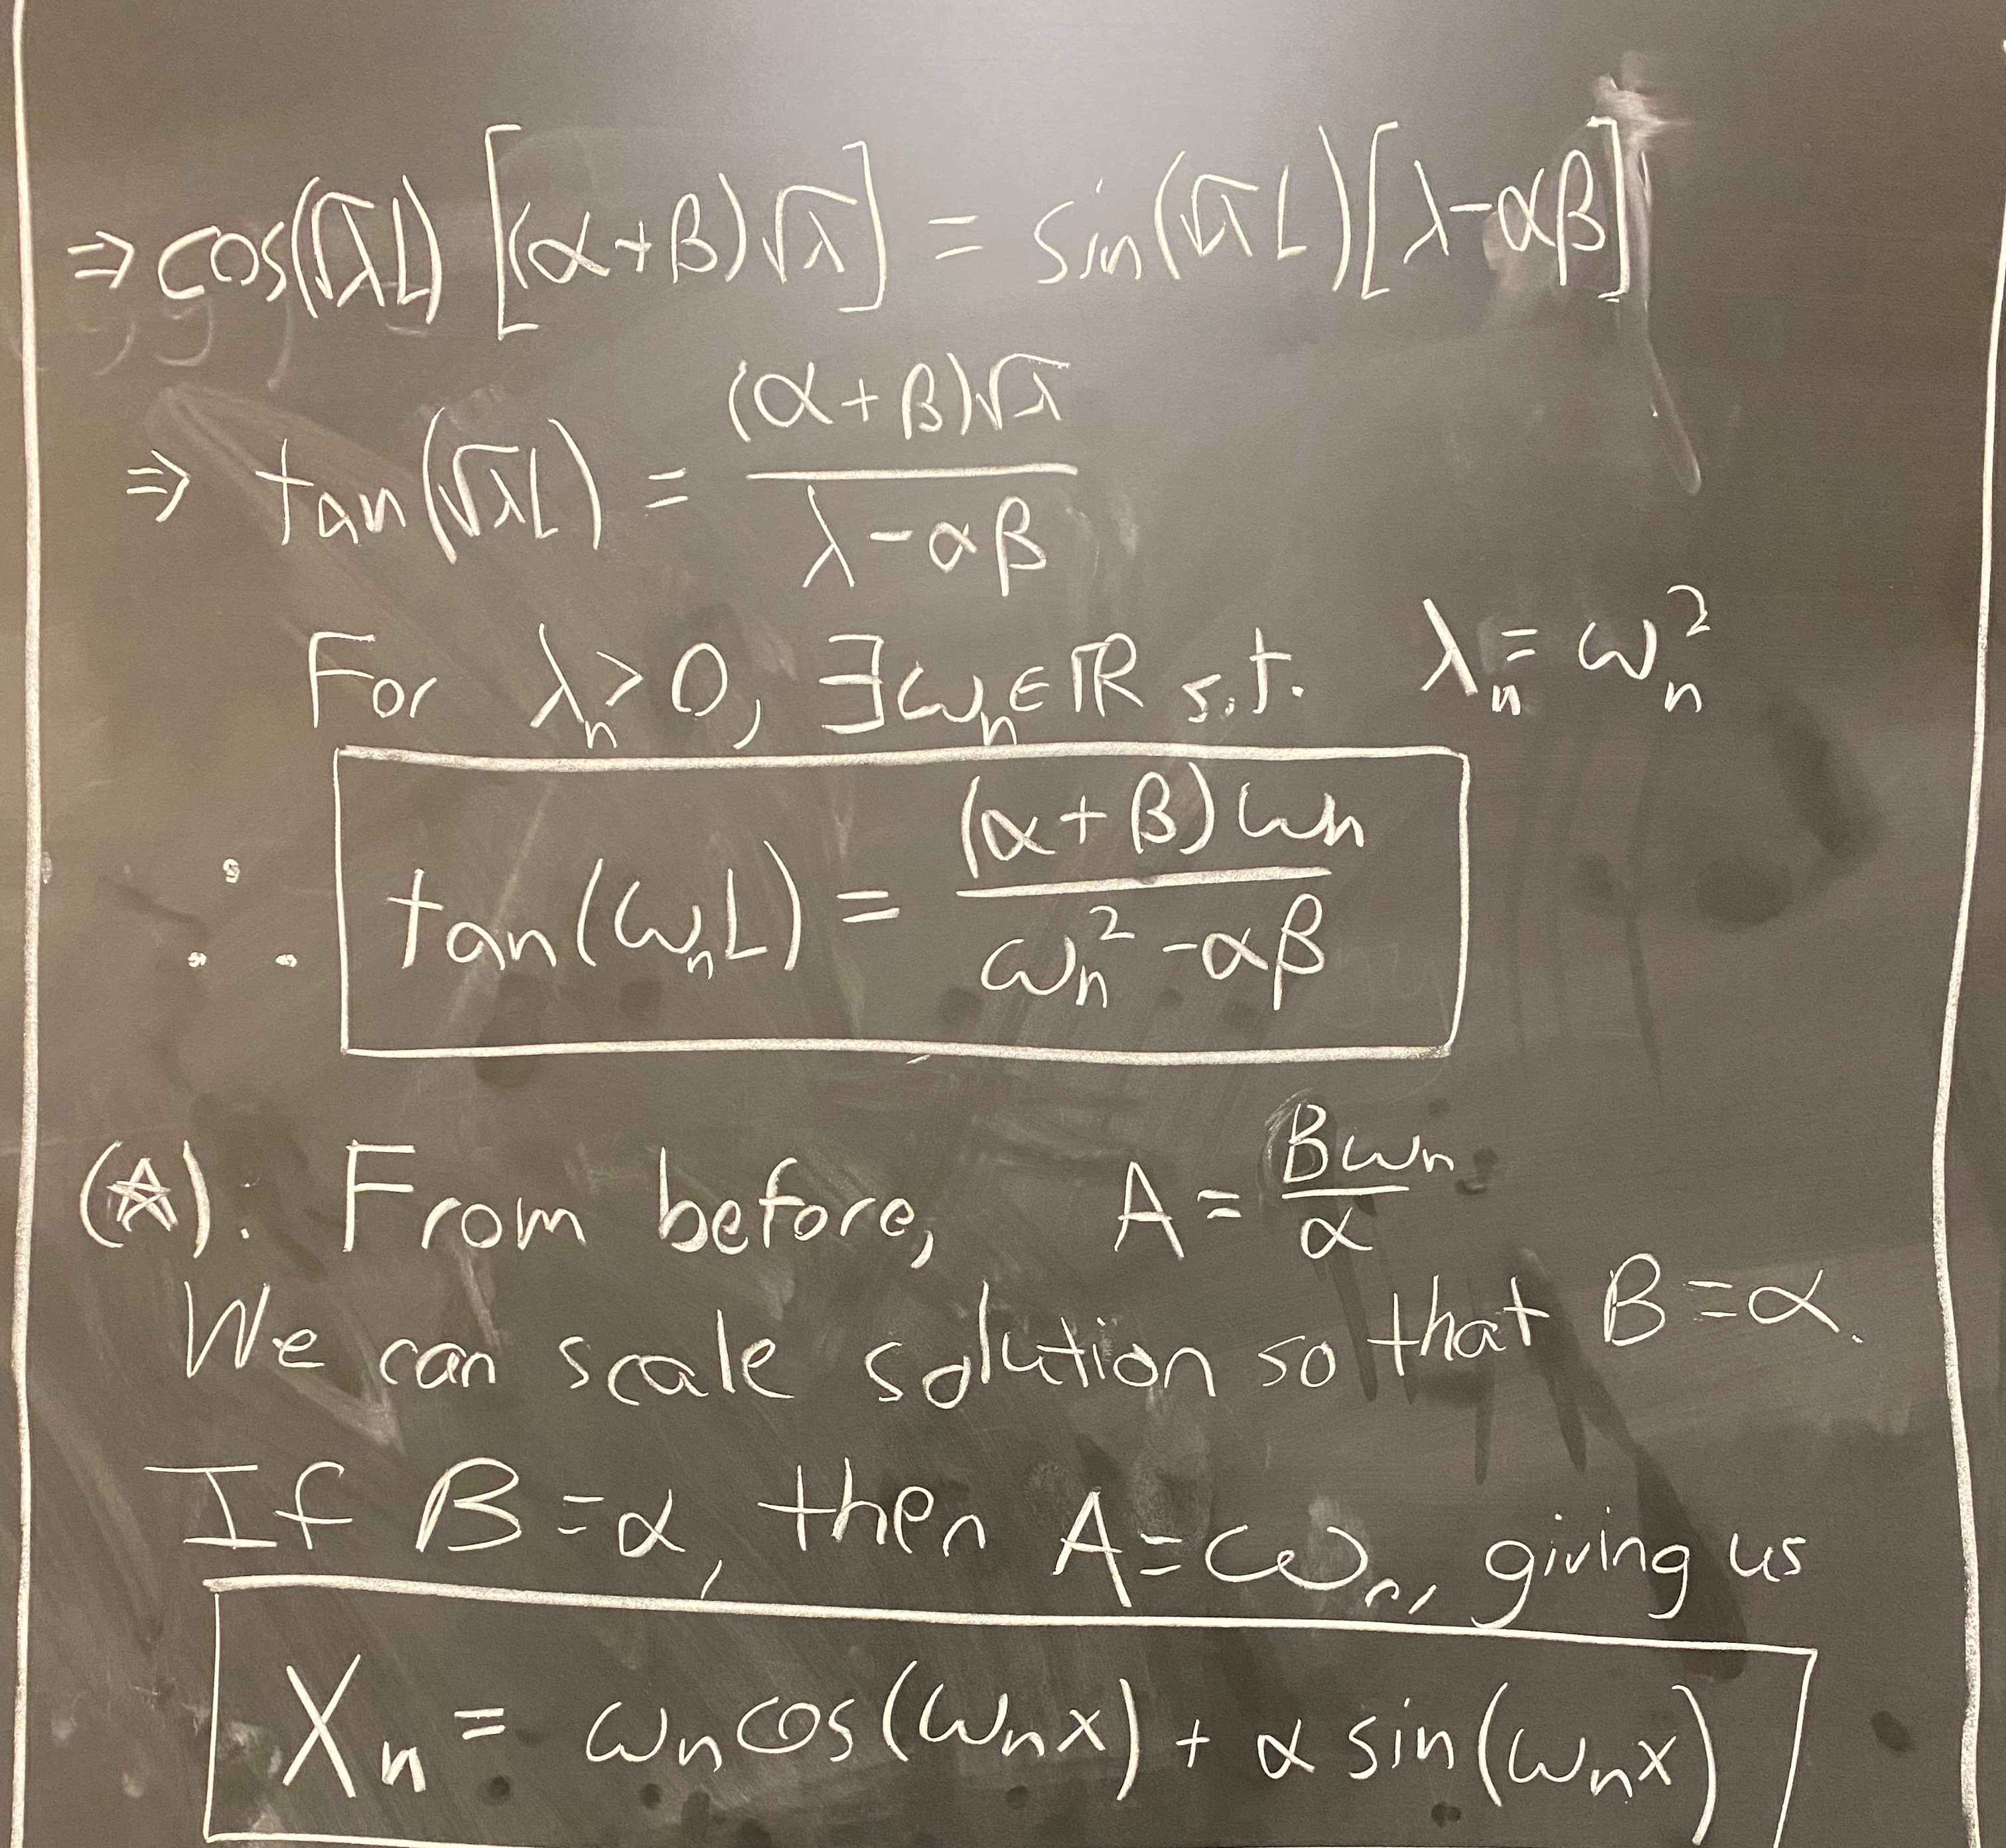
\includegraphics[width=0.3\textwidth]{Problem 1-1 (3).jpeg}
        \end{figure}

        \item \phantom{.}
        \begin{figure}[H]
            \centering
            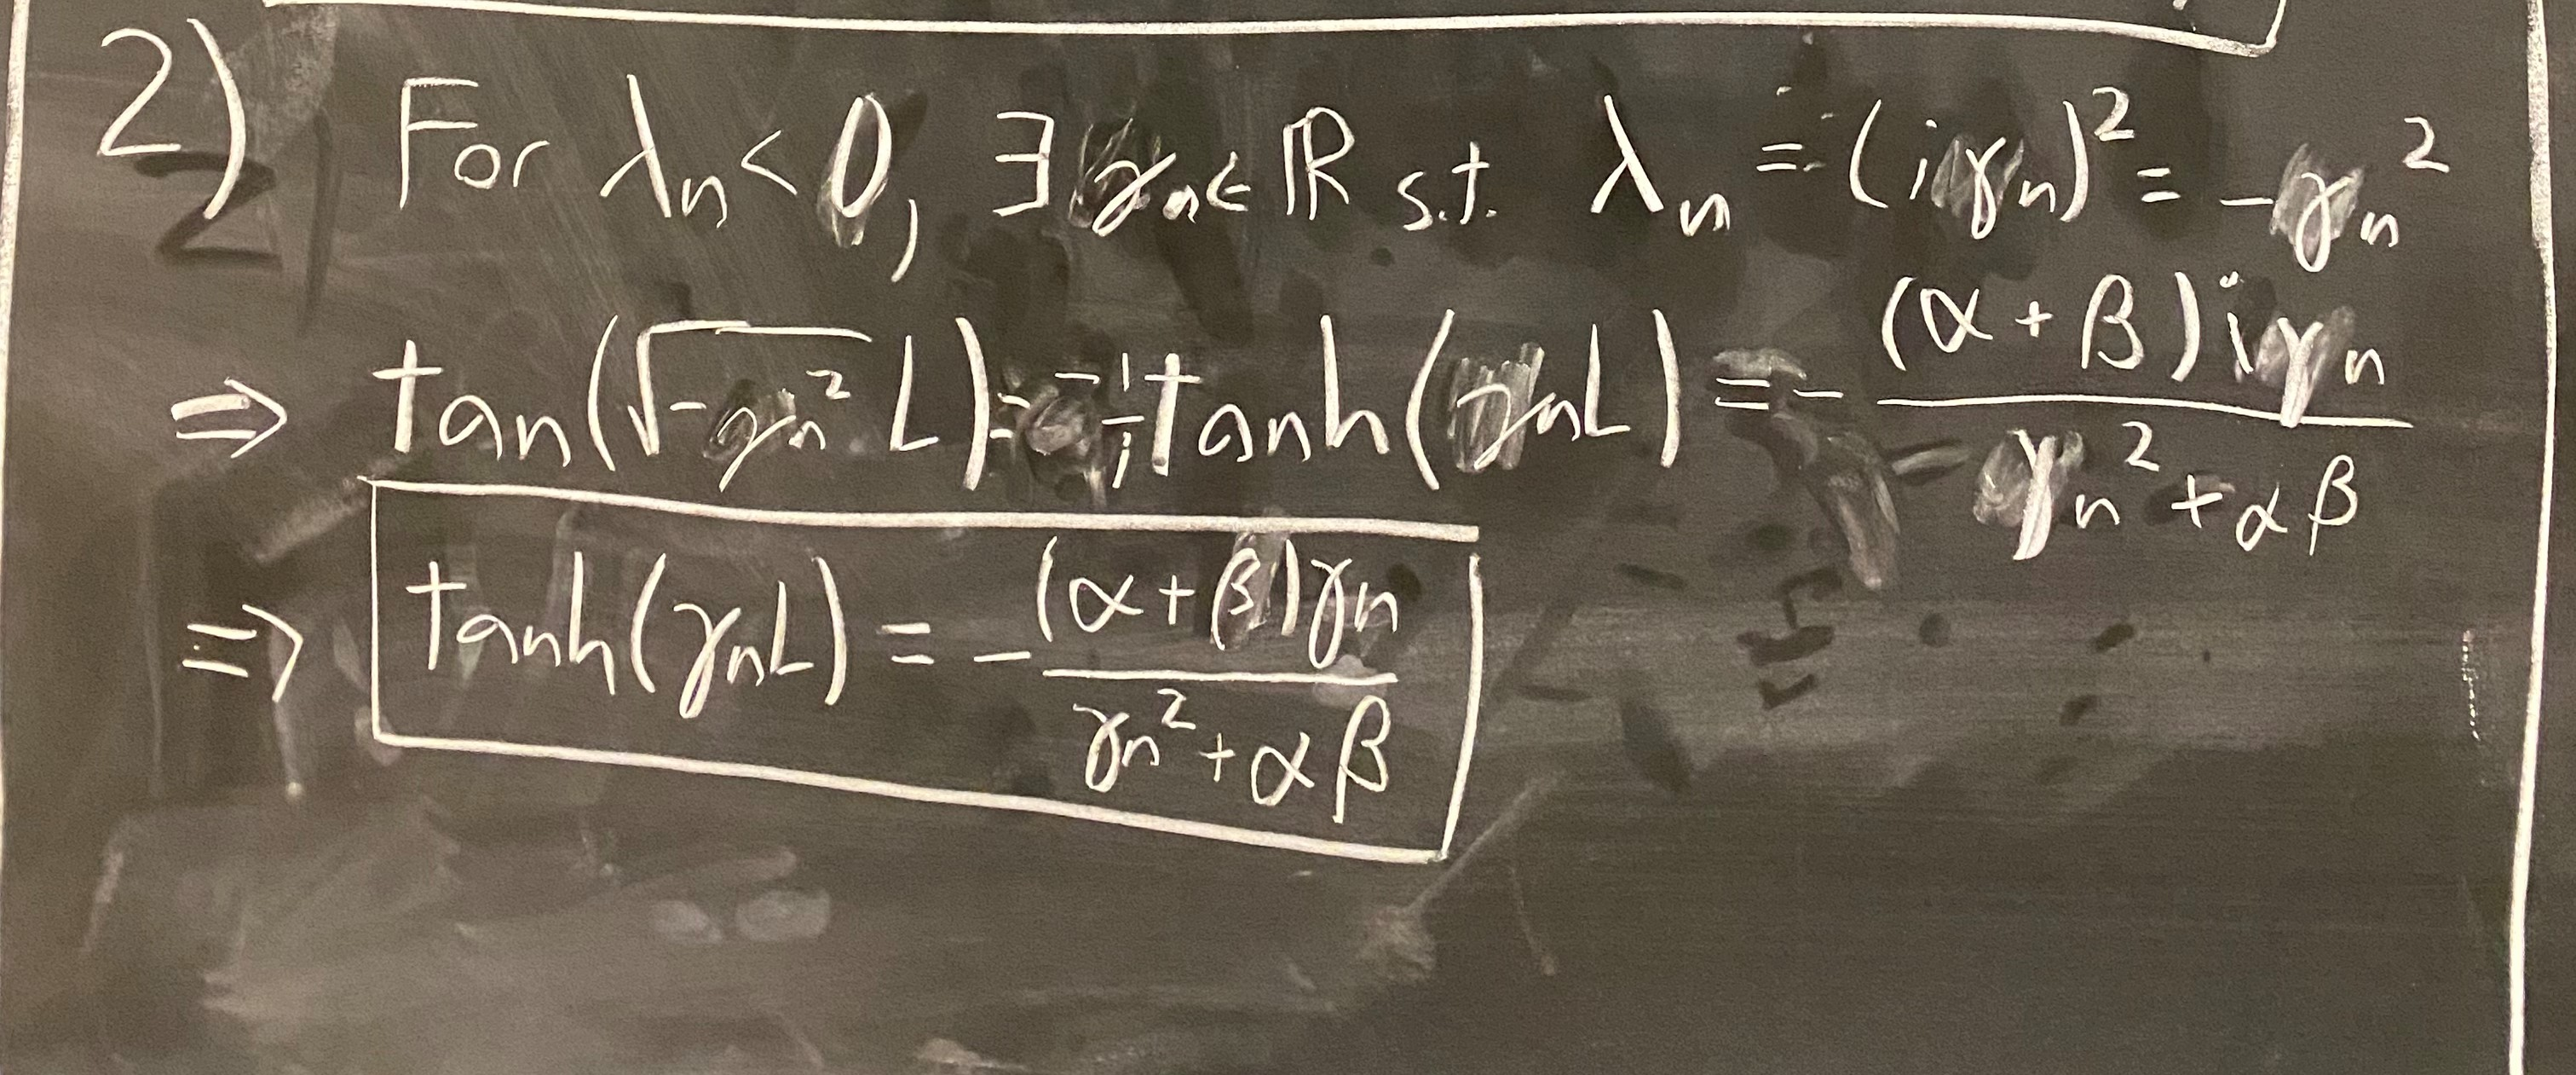
\includegraphics[height=1.5 in]{Problem 1-2.jpeg}
            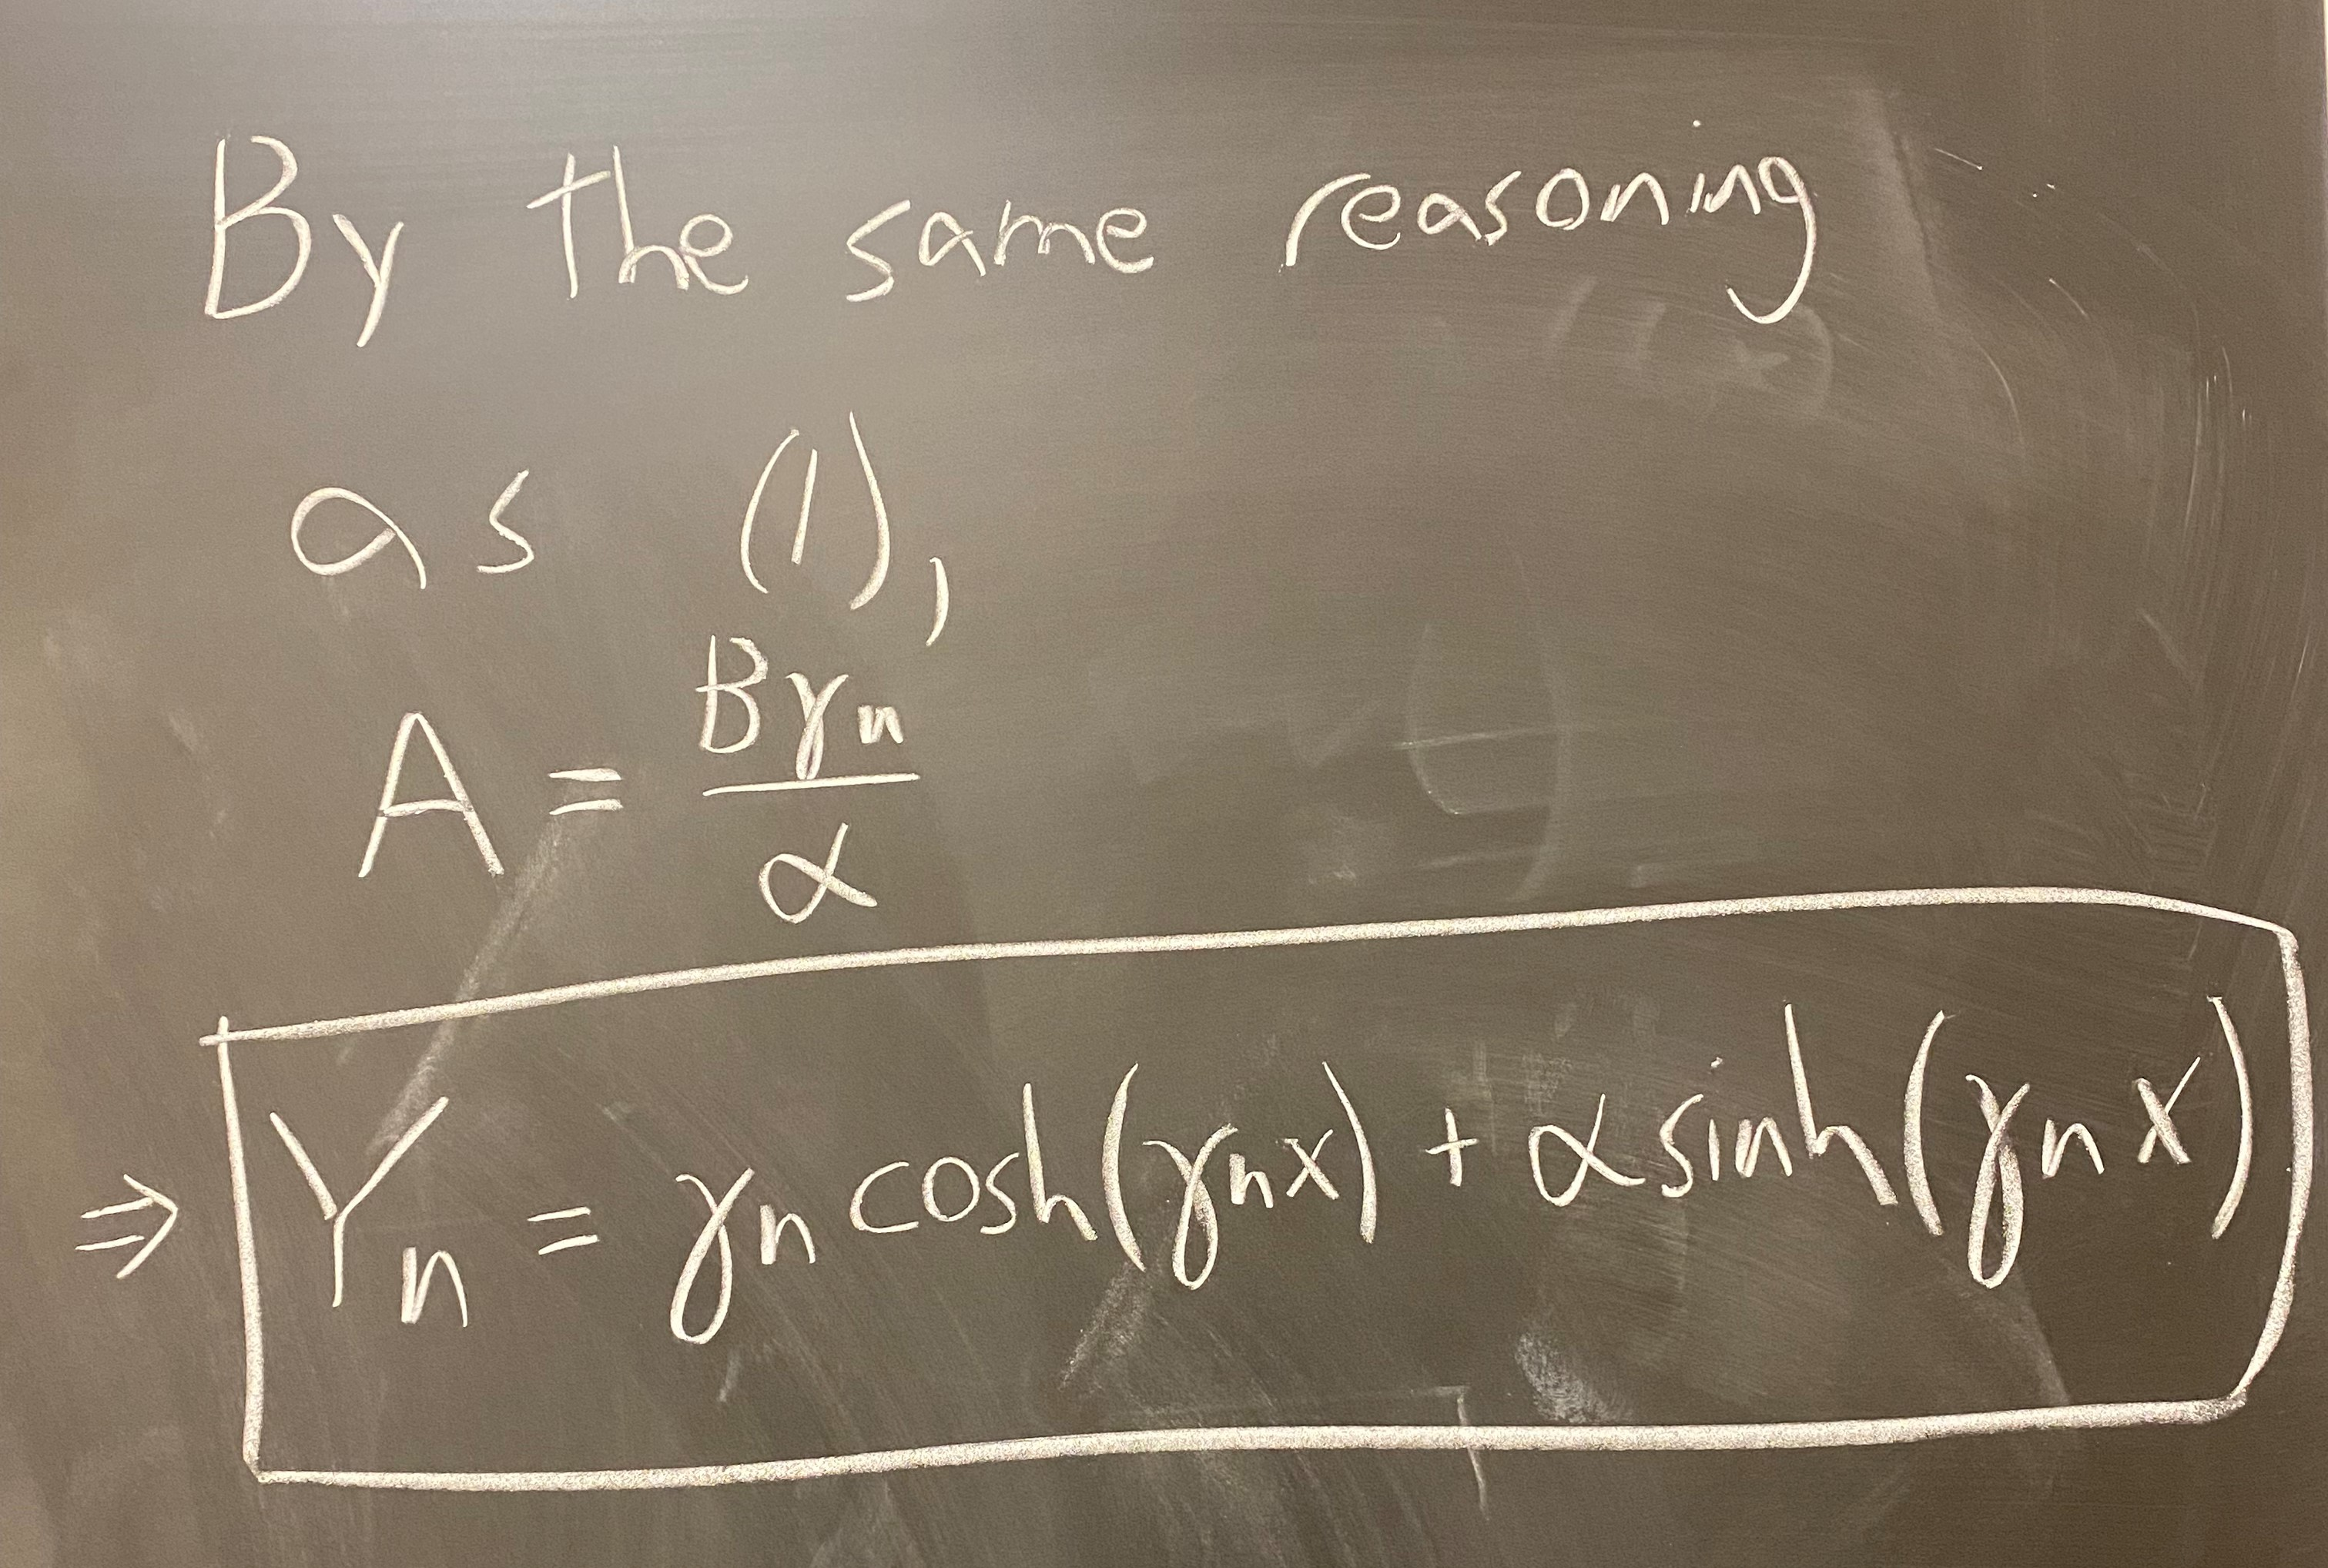
\includegraphics[height = 1.5 in]{Problem 1-2 (2).jpeg}
        \end{figure}

        \item \phantom{.}
        \begin{figure}[H]
            \centering
            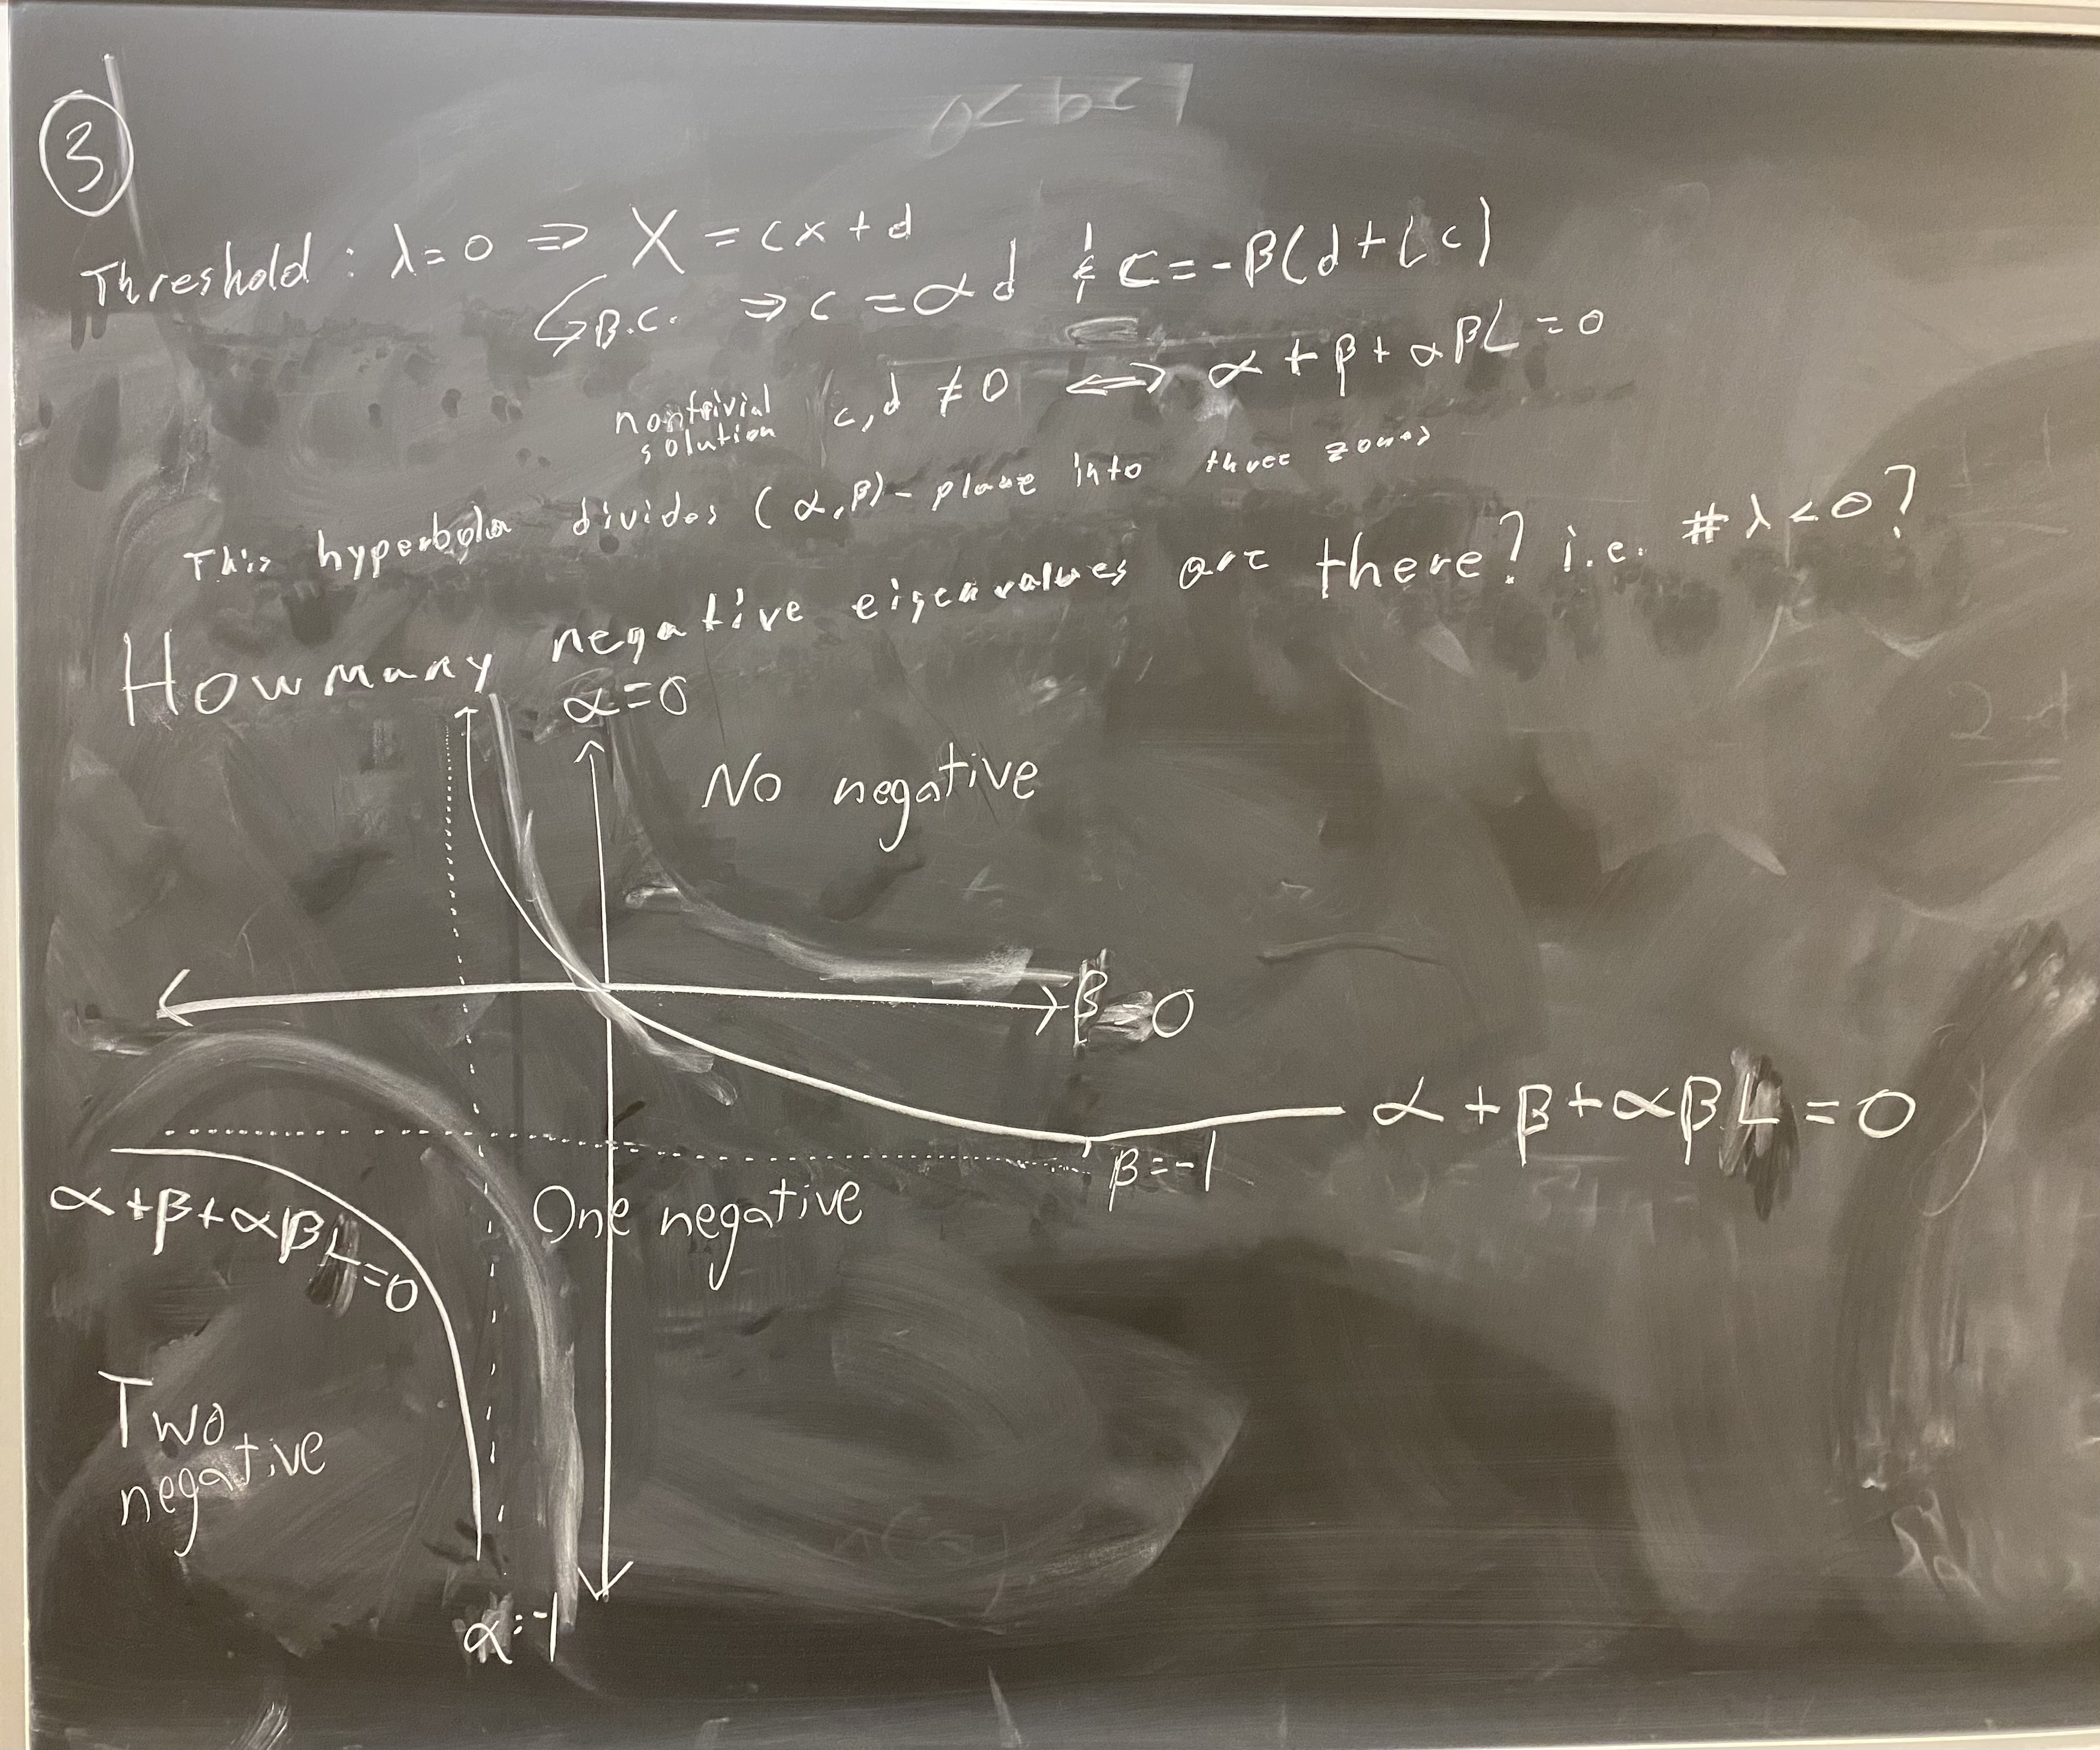
\includegraphics[width=0.7\textwidth]{Problem 1-3.jpeg}
        \end{figure}

        \item \phantom{.}
        \begin{figure}[H]
            \centering
            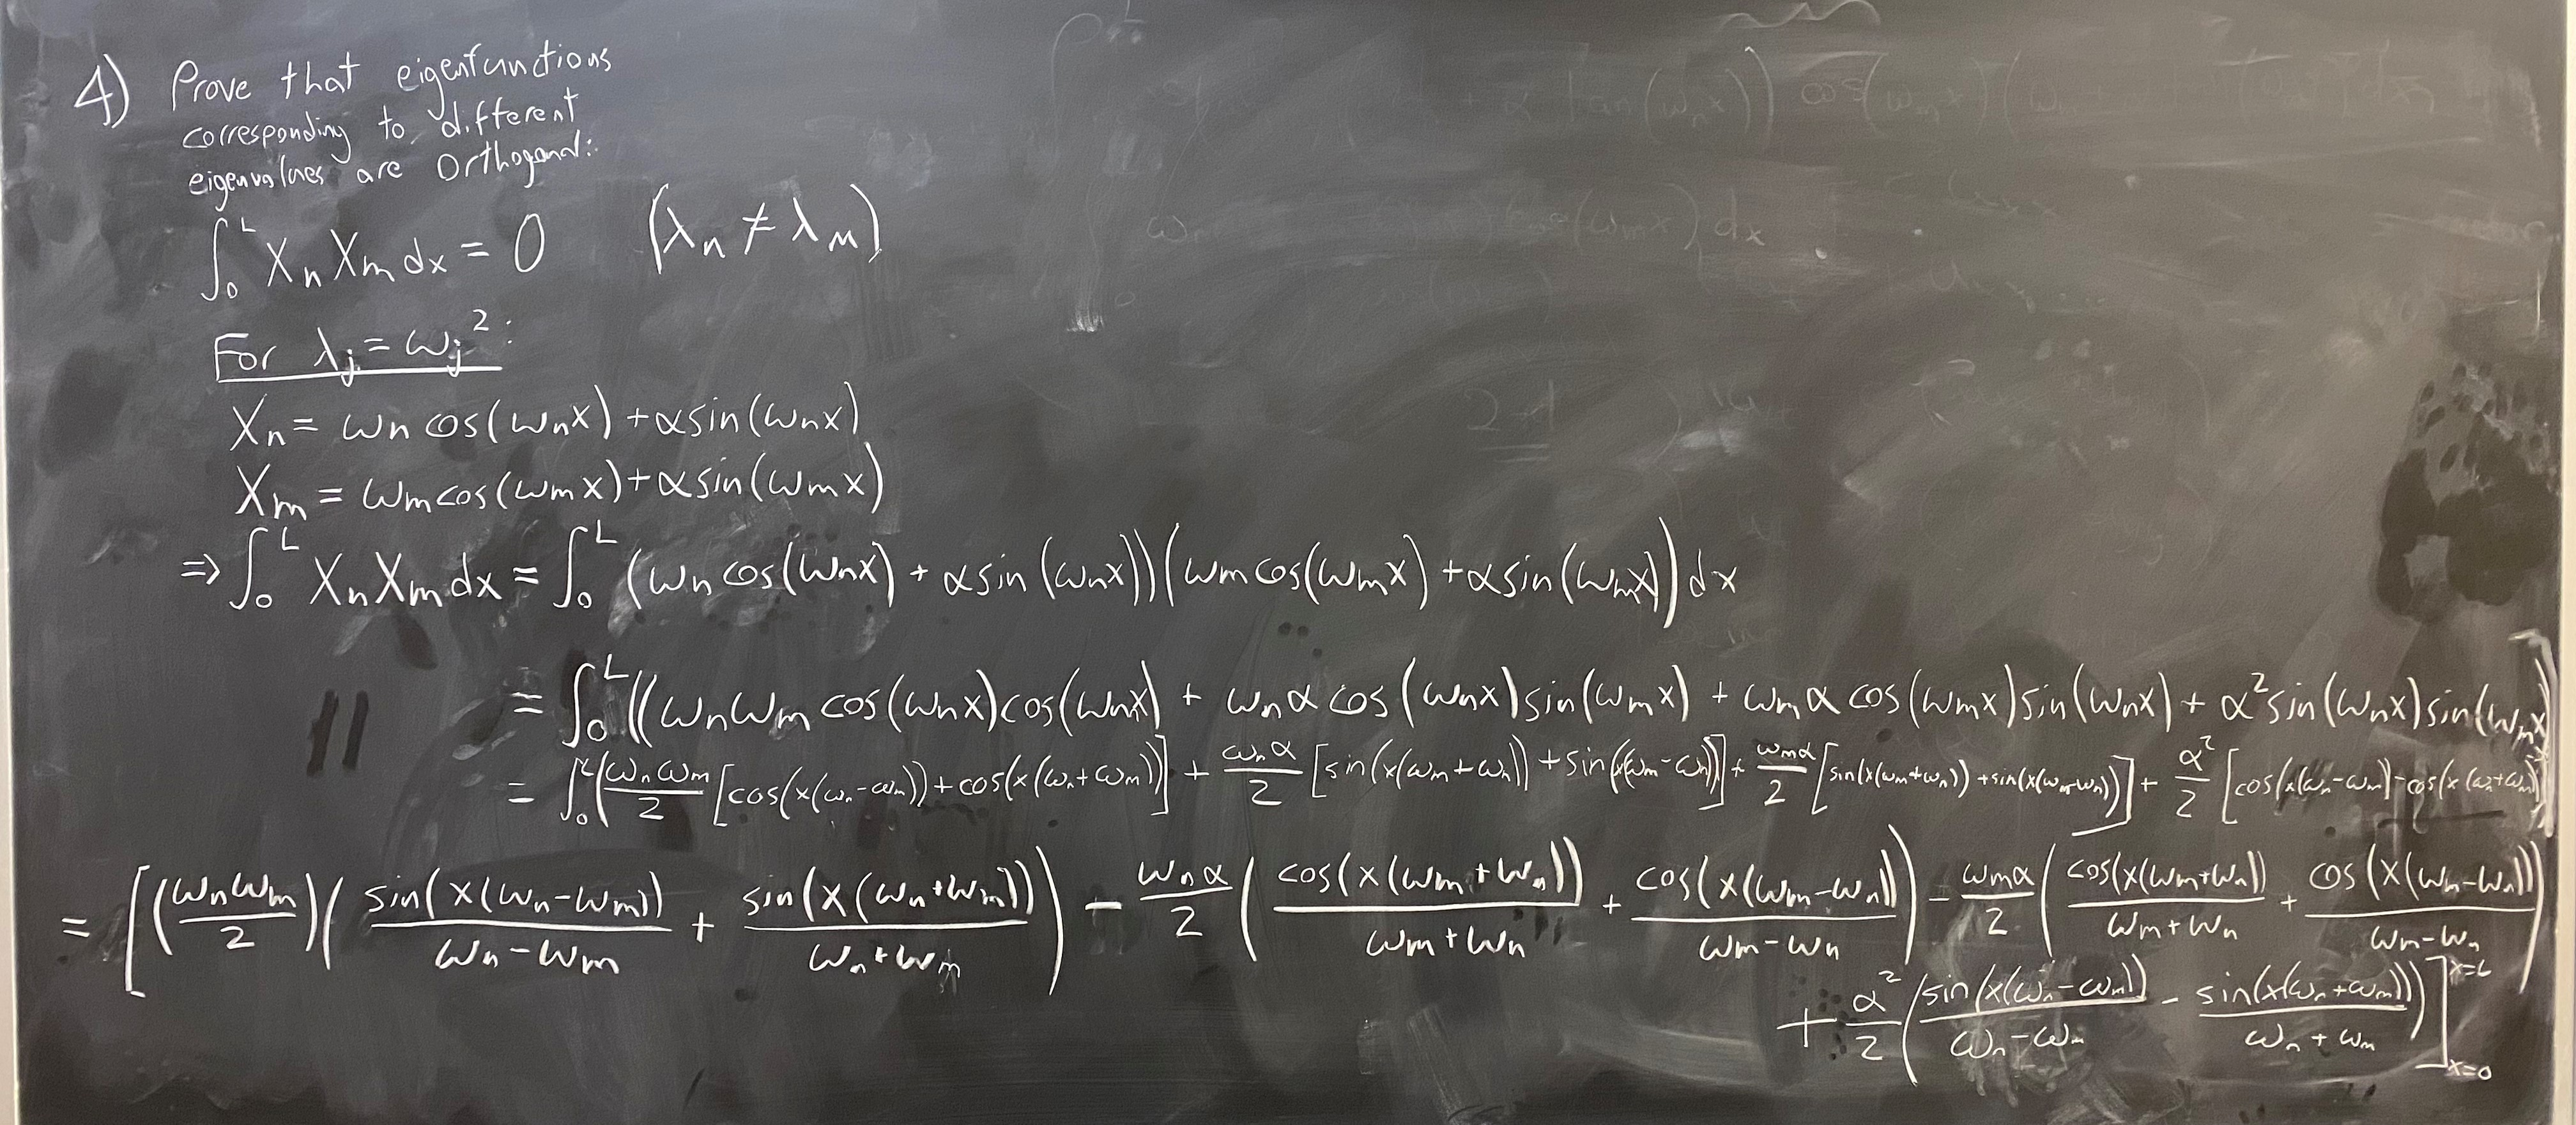
\includegraphics[width=\textwidth]{Problem 1-4.jpeg}
            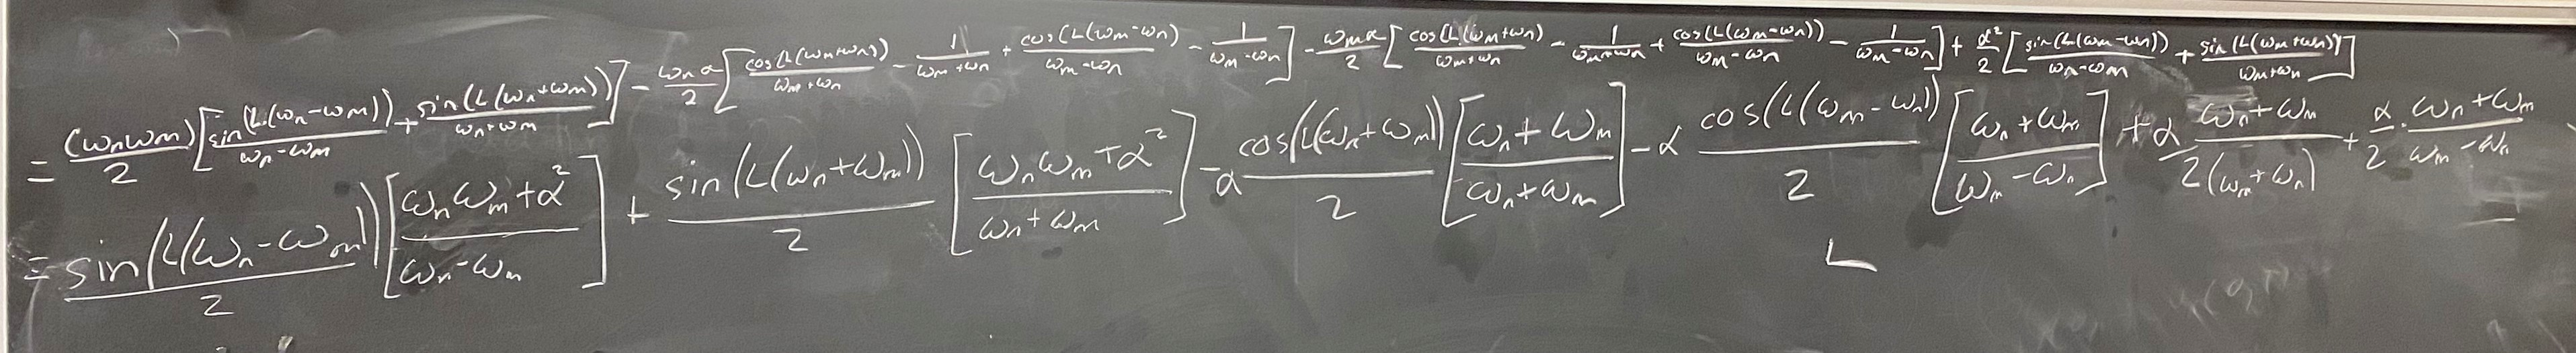
\includegraphics[width=\textwidth]{Problem 1-4 (2).jpeg}
        \end{figure}

    \end{enumerate}
\end{ans}

\begin{boldenv}
    \underline{Problem 3}. Oscillations of the beam are described by equation
    \[ u_{tt} + Ku_{xxxx} = 0. \mkern 50mu 0<x<l \]
    with $K > 0$.
    If both ends clamped (that means having the fixed positions and directions) then the boundary conditions are \begin{align*}
        &u(0,t) = u_x(0,t)=0\\
        &u(l,t) = u_x(l,t)=0
    \end{align*} \begin{enumerate}
        \item Find equation, describing frequencies, and find corresponding eigenfunctions (You may assume that all eigenvalues are real and positive).

        \item Solve equation, describing frequencies, graphically.
    \end{enumerate}
    \textit{Hint.} One can change coordinate system so that interval becomes $[-L, L] \text{ with } L = \frac{l}{2}$ and then consider separately even and odd eigenfunctions.
\end{boldenv}
\begin{ans} \phantom{.}
    \begin{figure}[H]
        \centering
        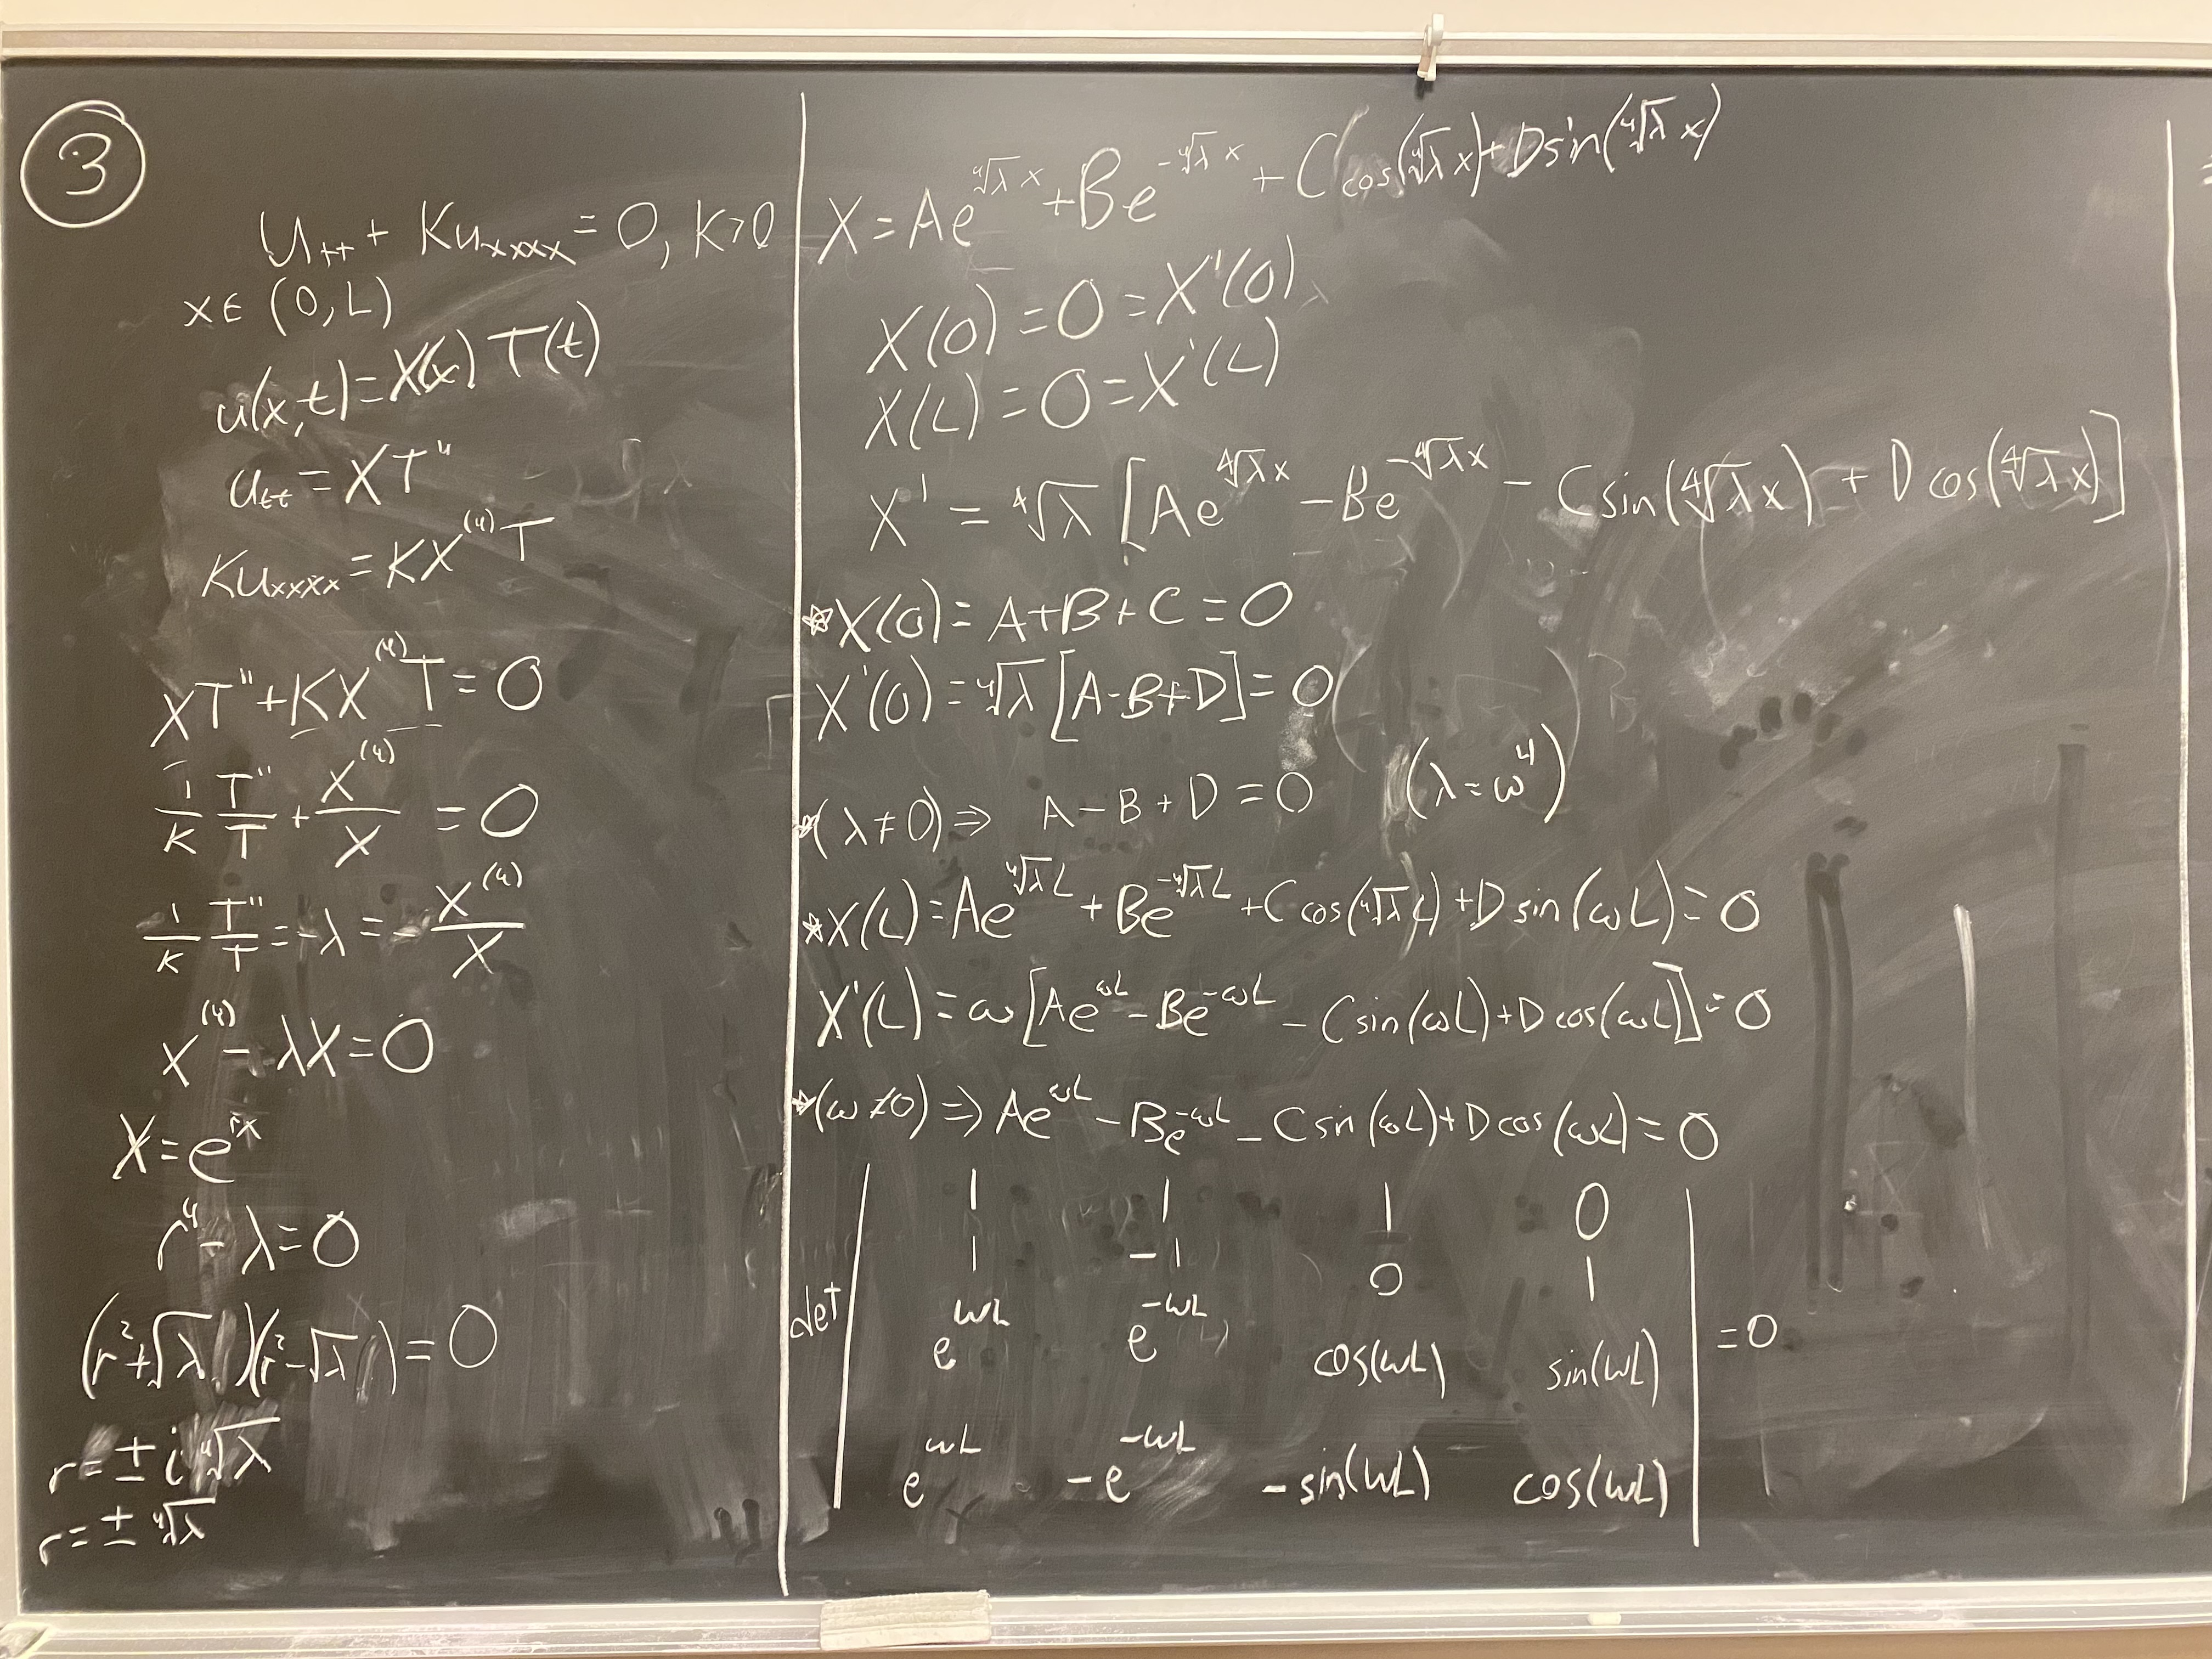
\includegraphics[width=0.9\textwidth]{Problem 3.jpg}
        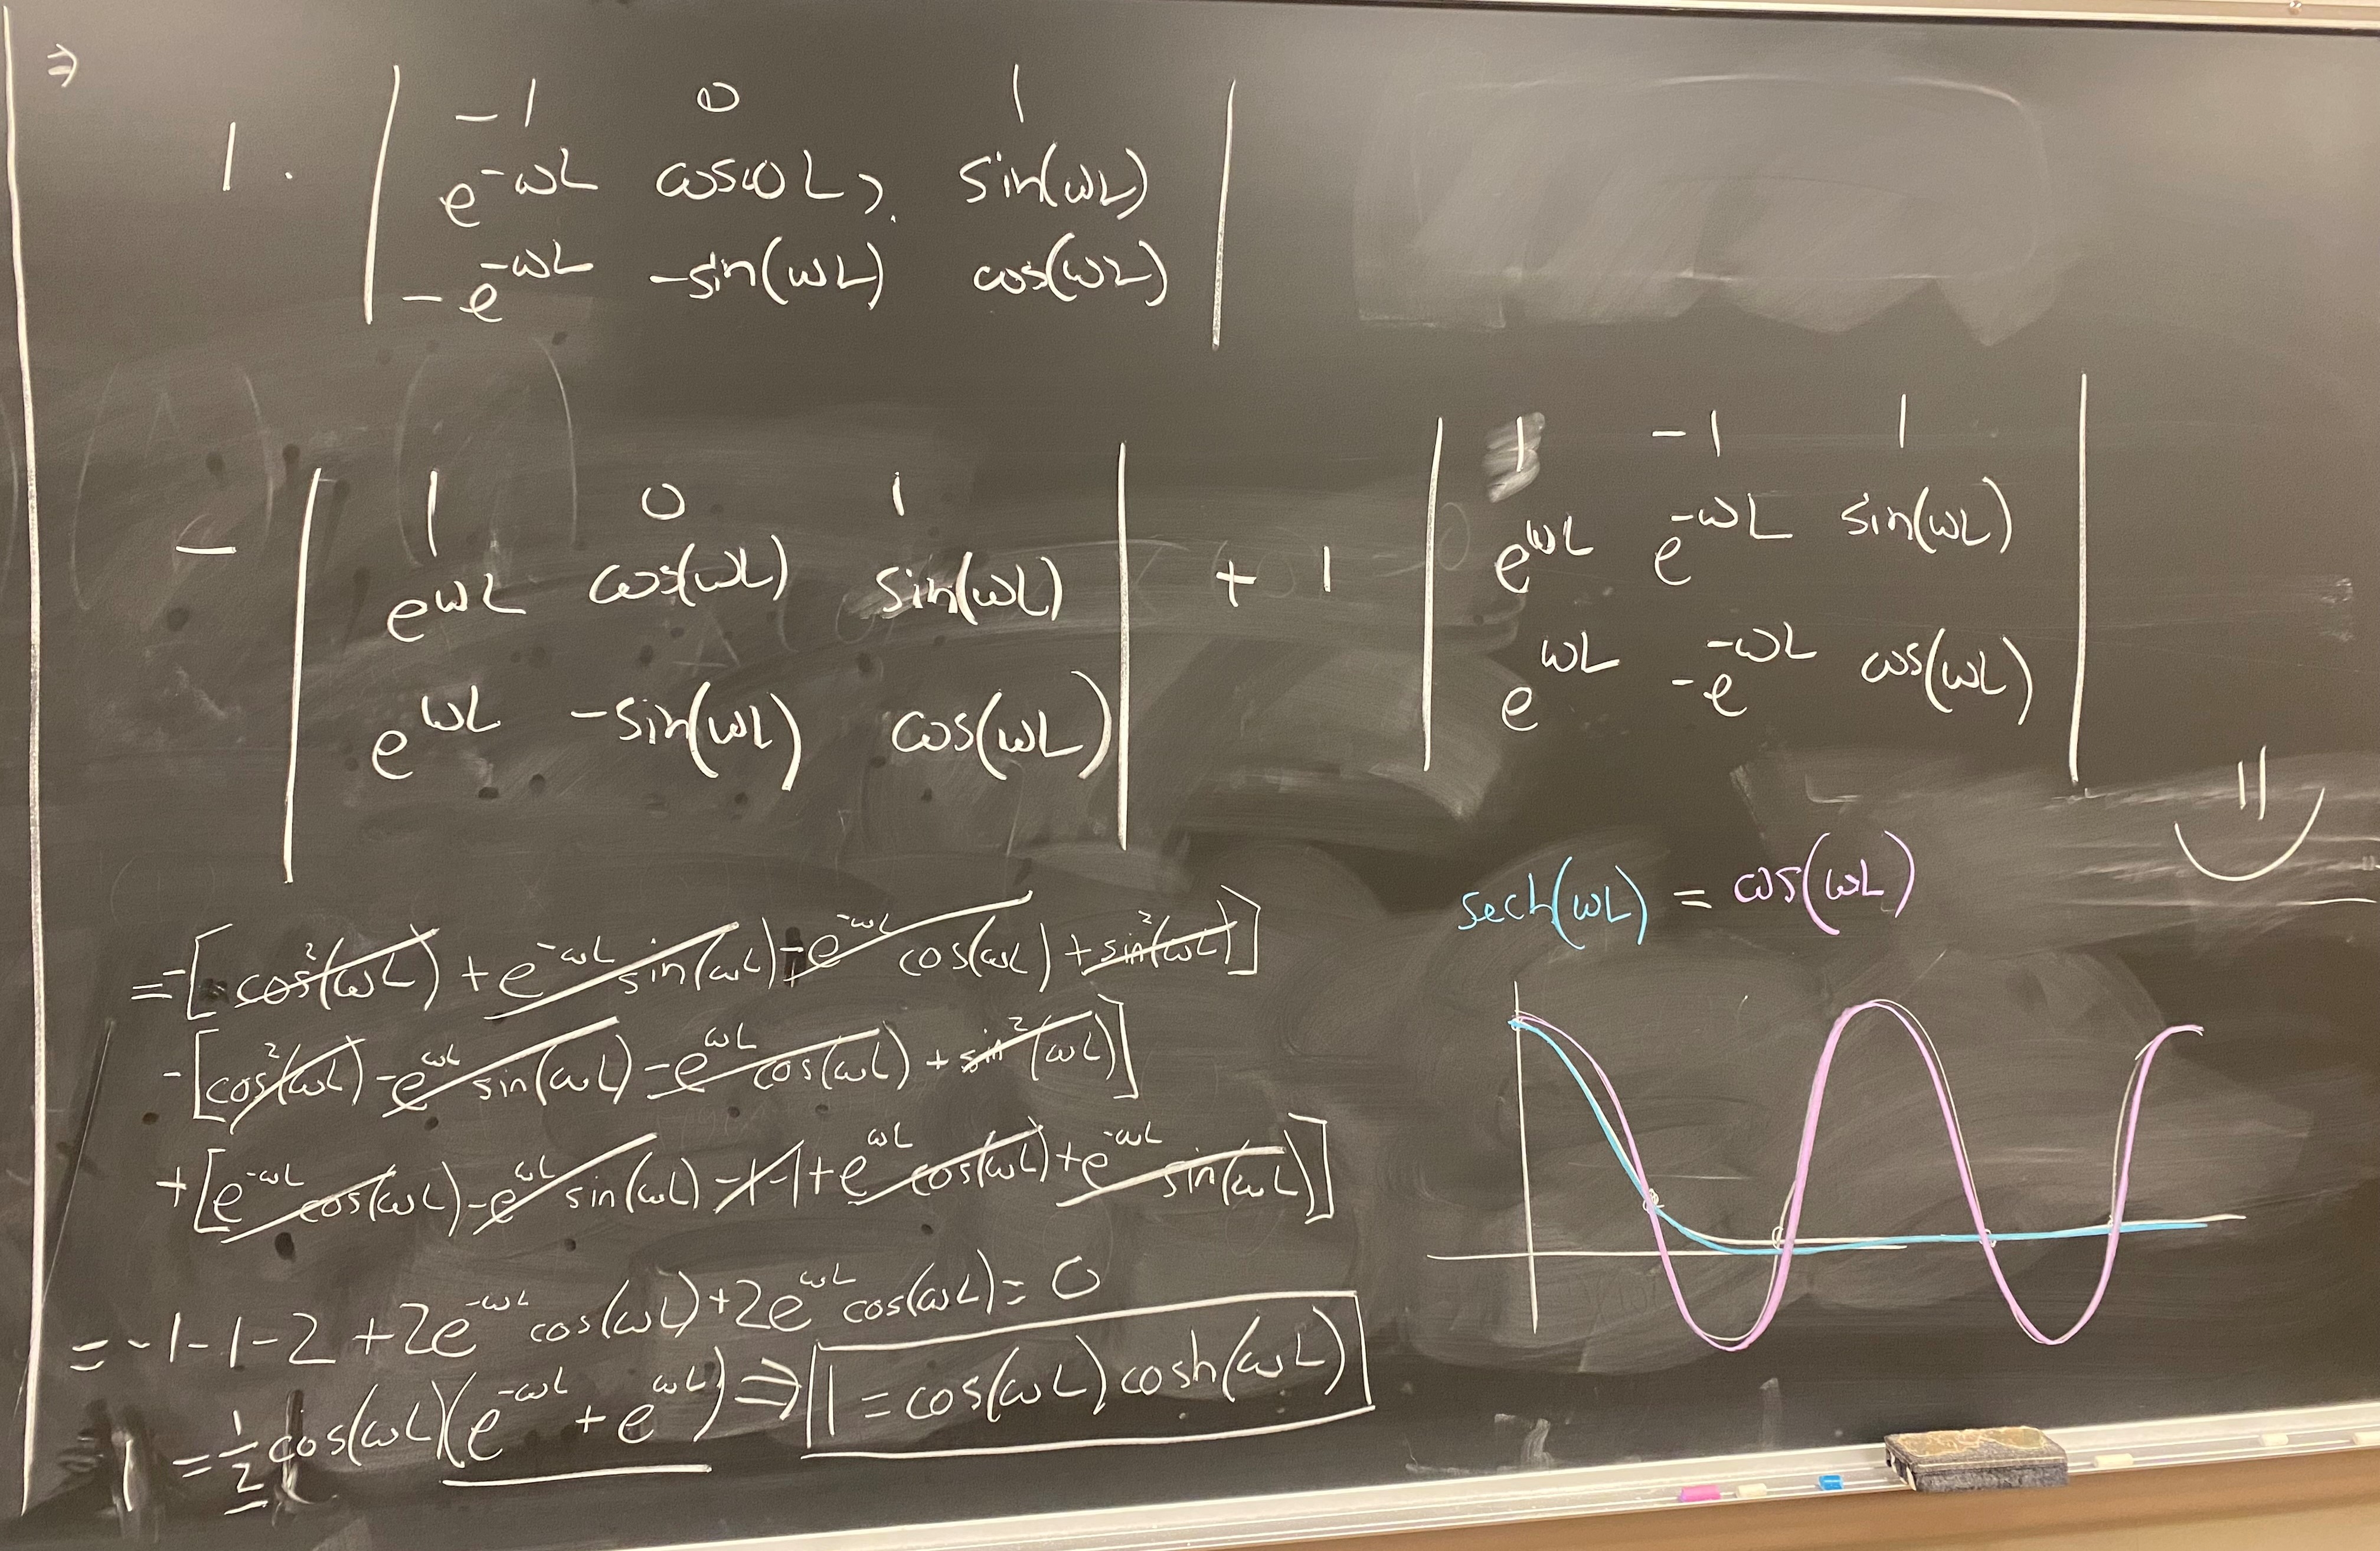
\includegraphics[width=0.9\textwidth]{Problem 3 (2).jpg}
    \end{figure}
\end{ans}
\newpage
\begin{boldenv}
    \underline{Problem 9}. Consider wave equation with the Neumann boundary condition on the left and "weird" b.c. on the right: \begin{align*}
        &u_{tt} - c^2u_{xx} = 0 \mkern 50mu 0<x<l,\\
        &u_x(0,t) = 0,\\
        &(u_x + i\alpha u_t)(l,t) = 0
    \end{align*}
    with $\alpha \in \R$. \begin{enumerate}
        \item Separate variables;
        \item Find "weird" eigenvalue problem for ODE;
        \item Solve this problem;
        \item Find simple solution $u(x,t)=X(x)T(t)$.
    \end{enumerate}
    \textit{Hint.} You may assume that all eigenvalues are real (which is the case).
\end{boldenv}
\begin{ans} \phantom{.}
    \begin{figure}[H]
        \centering
        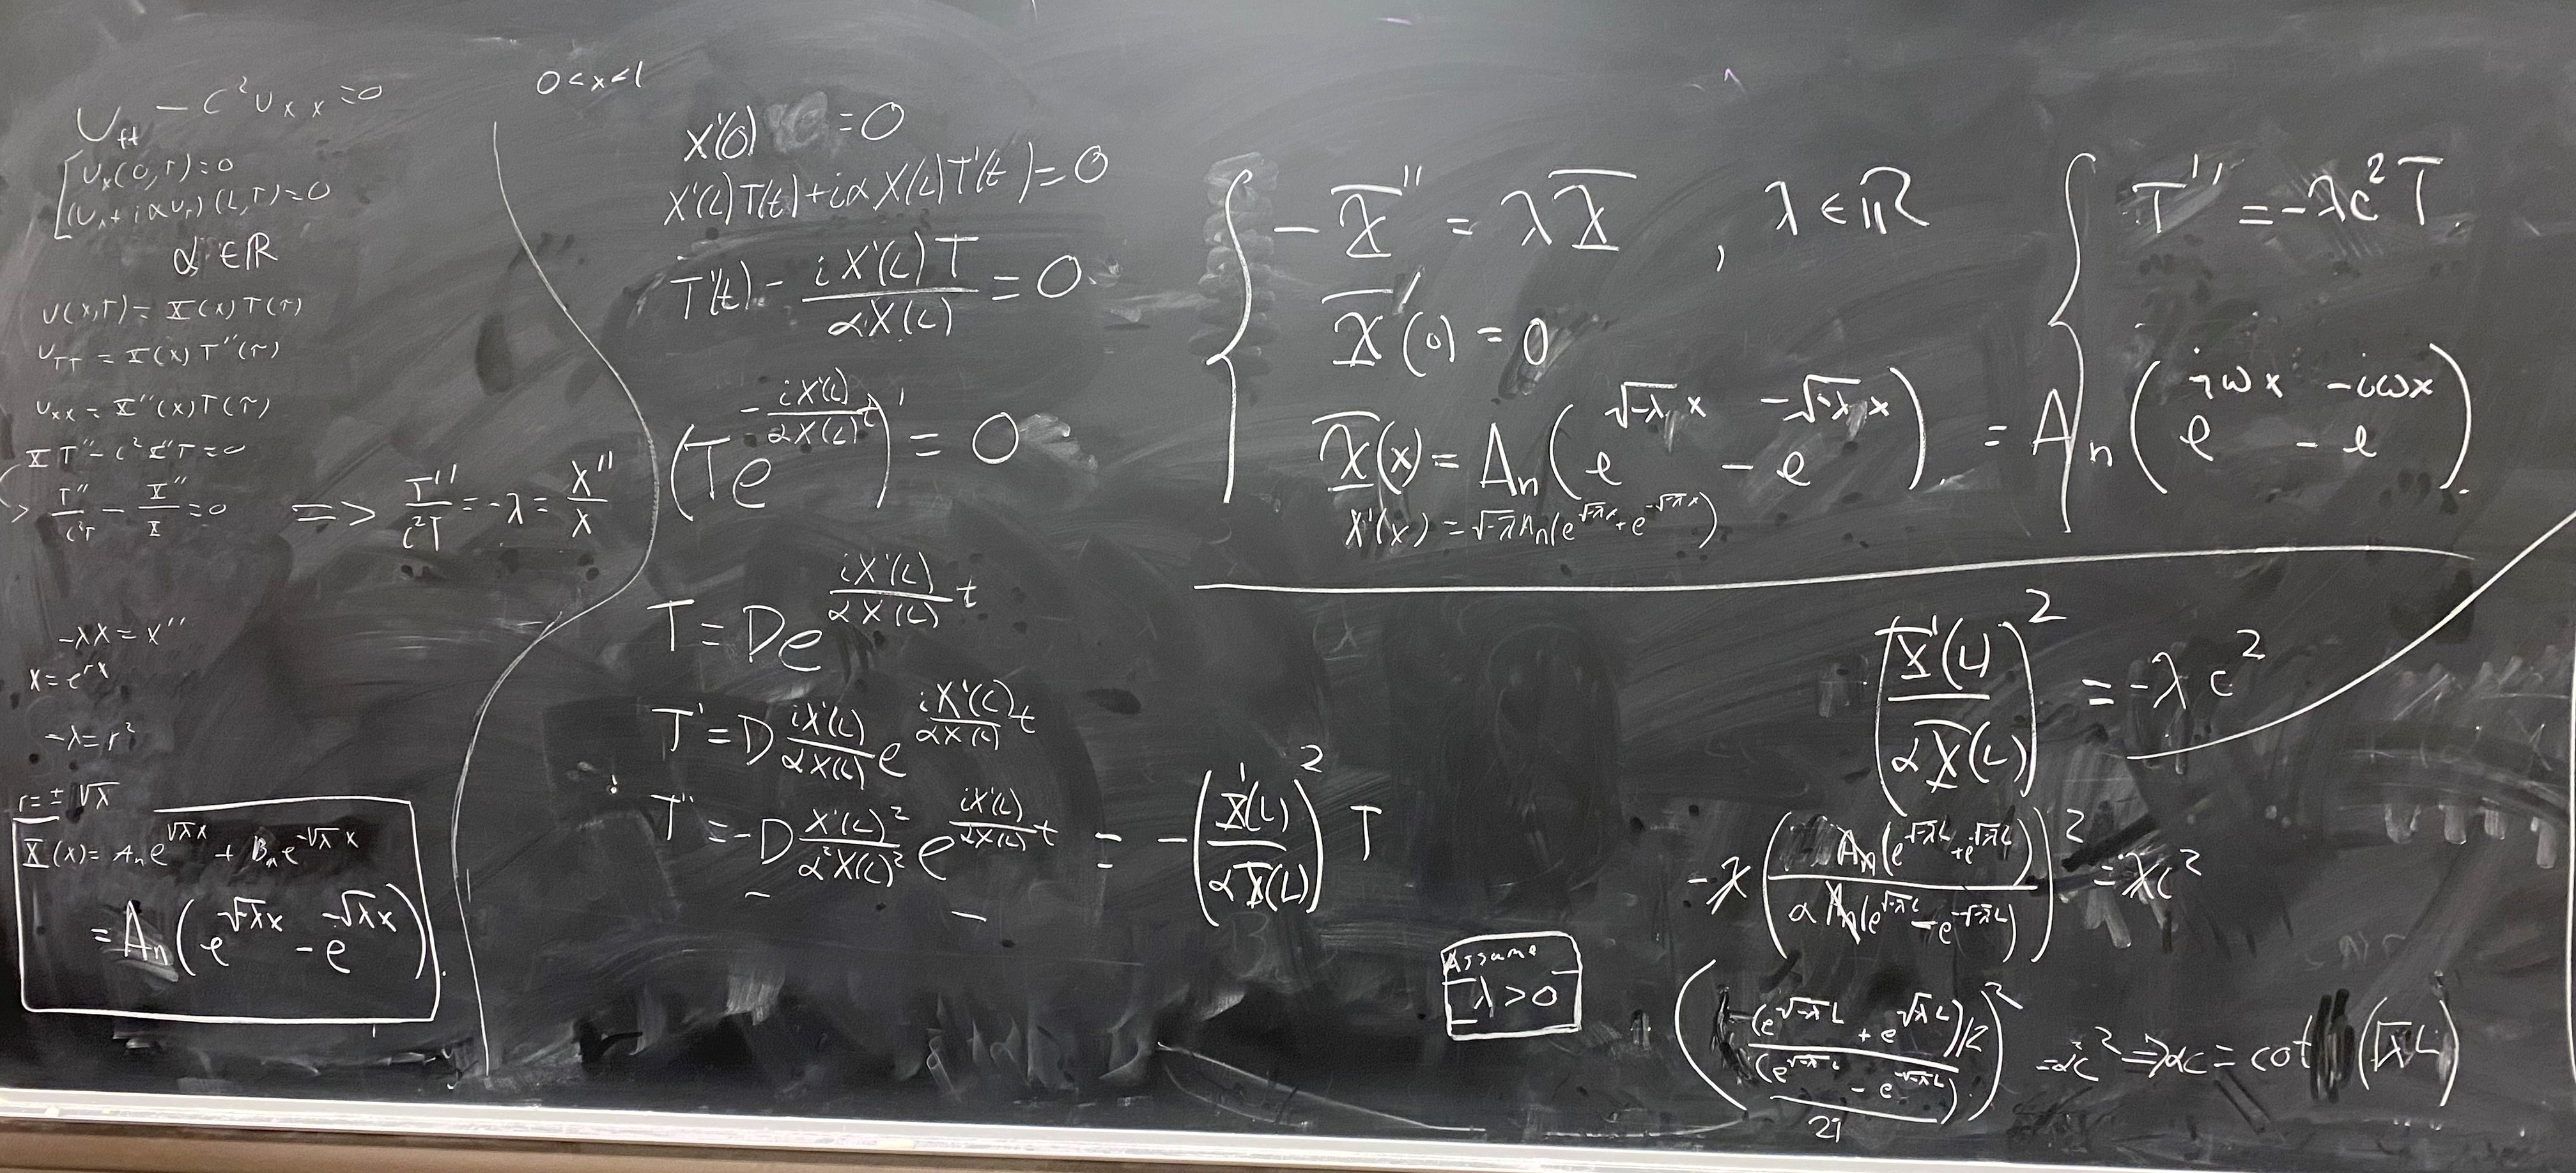
\includegraphics[width=\textwidth]{Problem 9.jpg}
        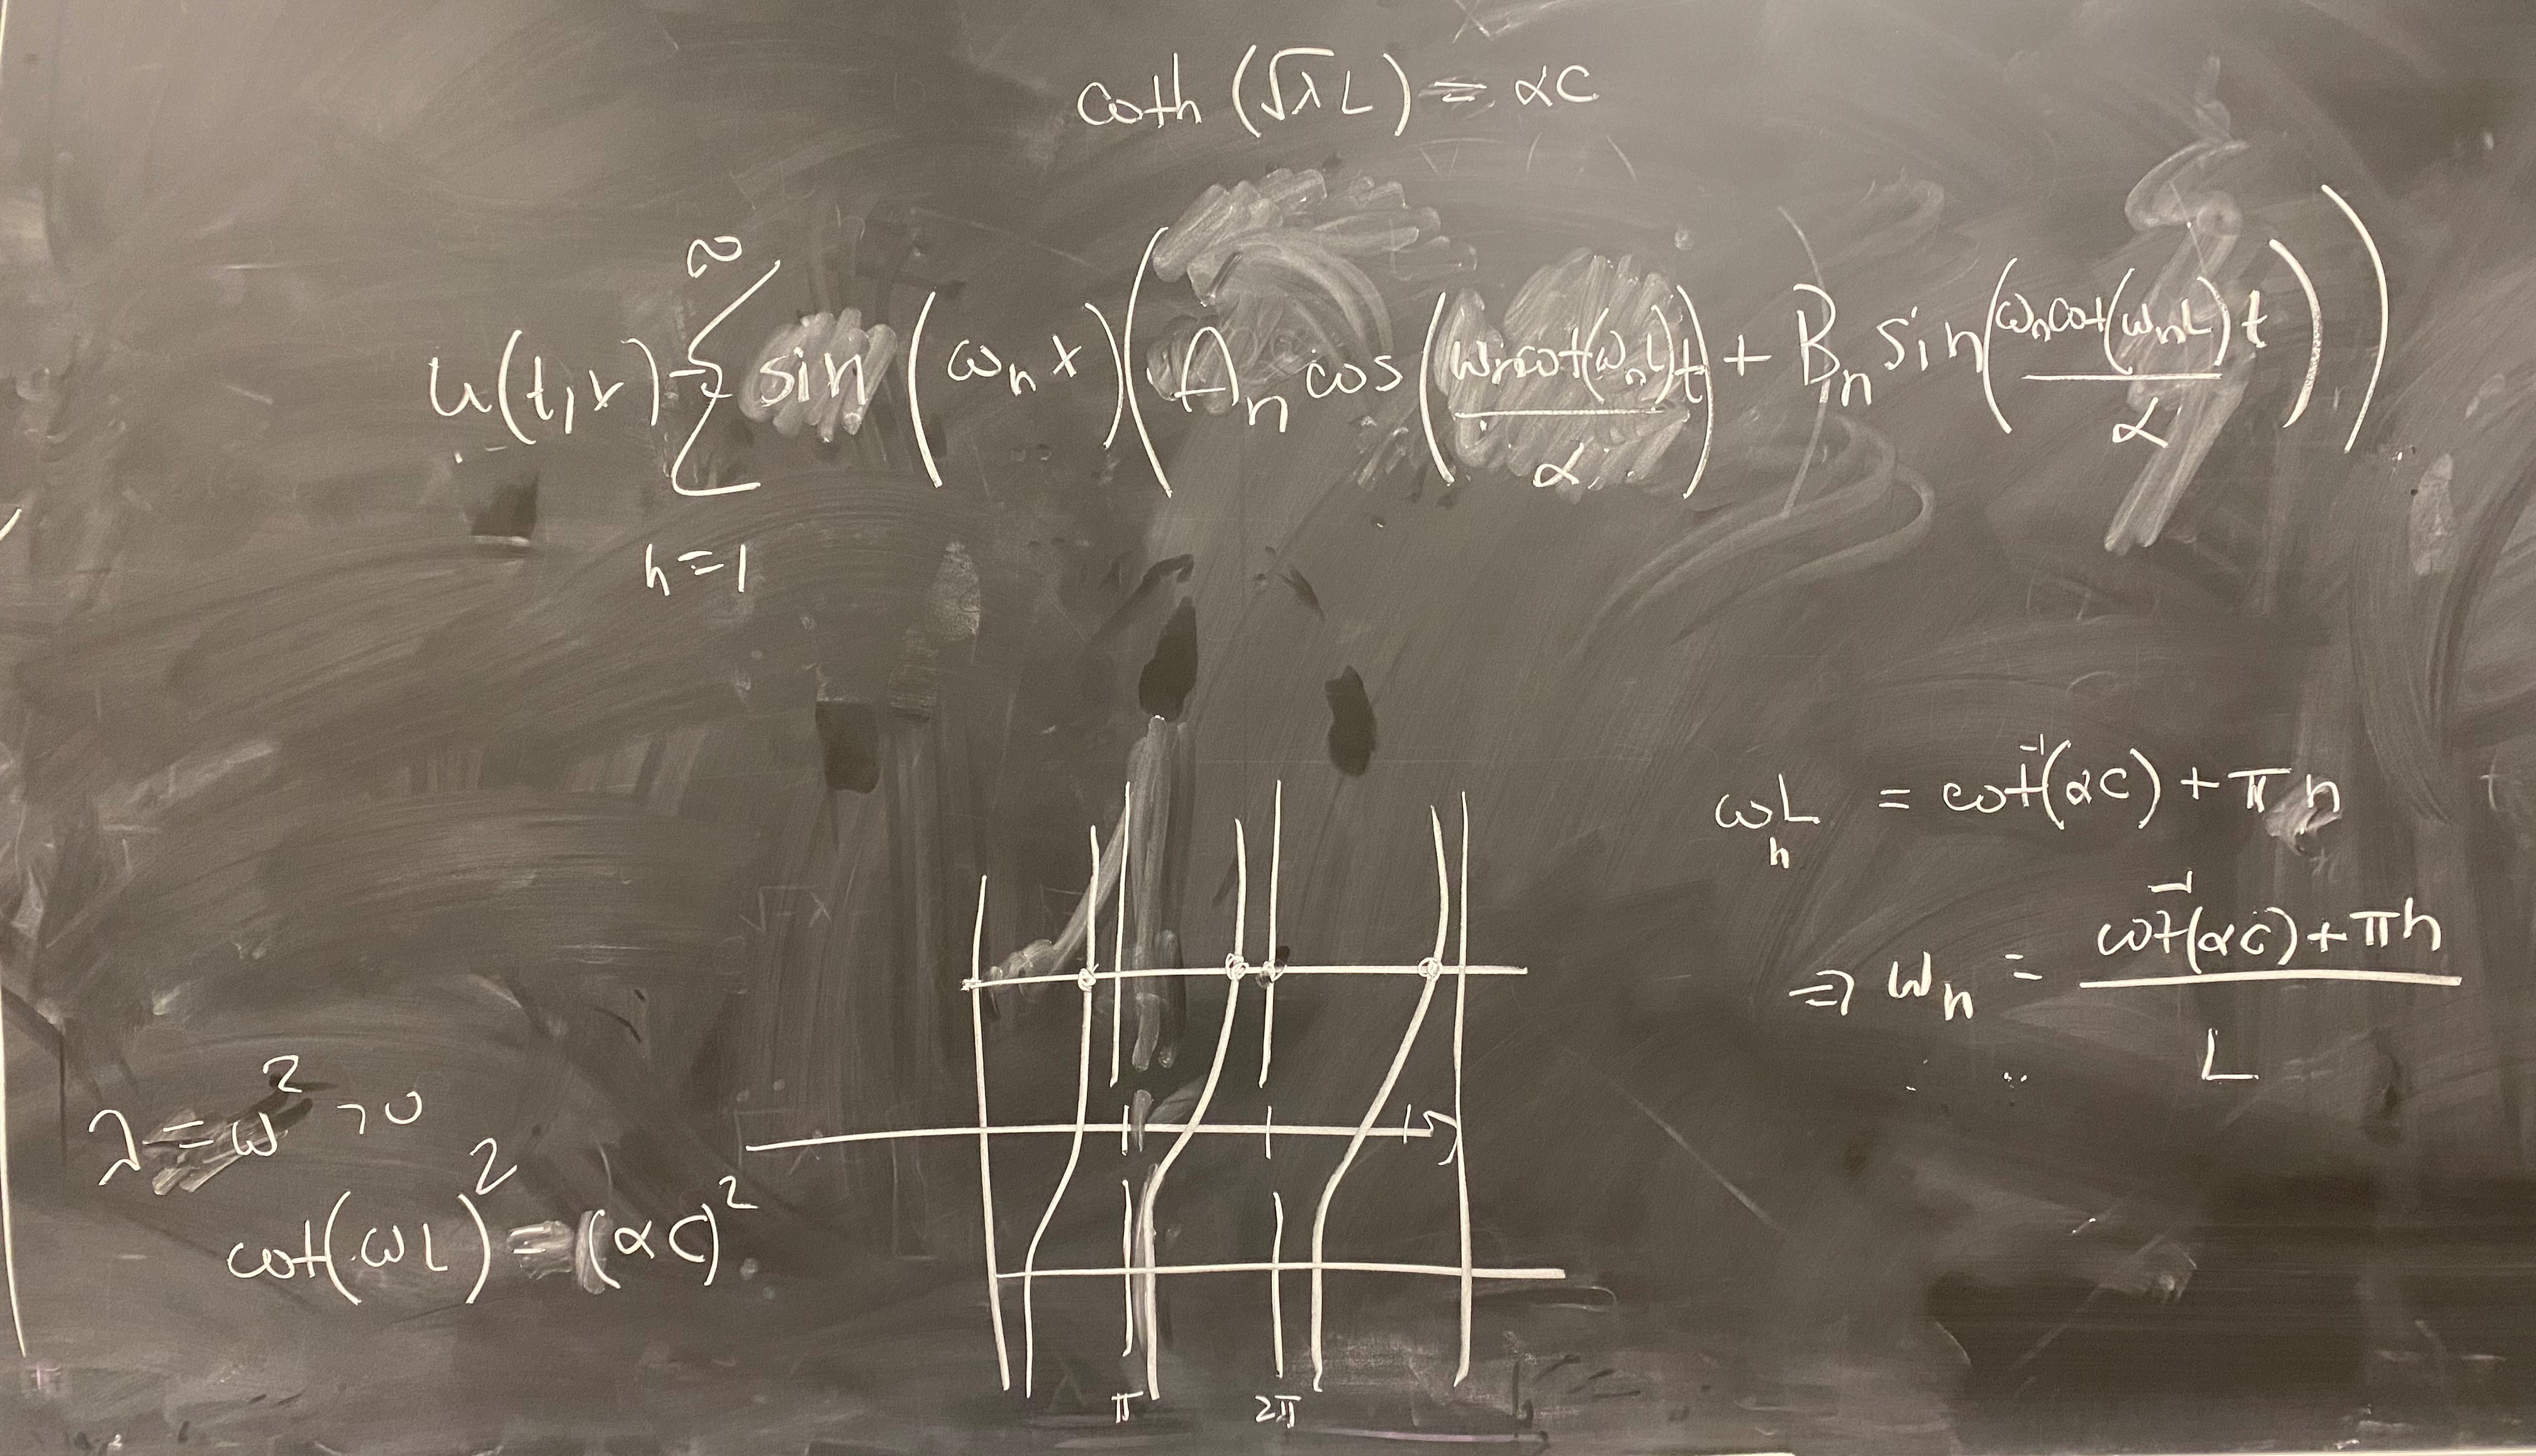
\includegraphics[width=0.7\textwidth]{Problem 9 (2).jpg}
    \end{figure}
\end{ans}

\end{document}
